\documentclass{article}
\usepackage{caption}
\usepackage{graphicx}
\usepackage{amsmath}
\usepackage{subcaption}
\usepackage{algorithm}
\usepackage{algpseudocode}

\title{Background and Specification Progress Report}
\author{Mohammad Ibrahim Khan}
\date{December, 2024}


\begin{document}
\maketitle

\tableofcontents
\listoffigures
\listoftables

\section{Background and Context}
\label{sec:background}

\subsection{Chess}
\label{sec:chess}
Modern chess is a game which had its origins in India, dating back to the 6th century \cite{davidsonShortHistoryChess2012}
as a way of devising strategy and tactics in war. Today it is a game seen as a benchmark for skill and 
intelligence, played by people in their millions. Some see chess as a way to relax while others 
see it as a sport, a competition \cite{averbakhHistoryChessChaturanga2012}.

\subsection{Chess Engines}
\label{sec:engines}
Since 1997 when IBM's Deep Blue beat Kasparov \cite{hsuIBMsDeepBlue1999}, a world champion, chess engines have been a 
popular topic of research. Chess engines analyse millions of positions per second in order to defeat
the best human players. However, even with technological advancements since 1997, chess is still
unsolved. According to Shannon, there are $10^{120}$ possible positions in chess \cite{shannonXXIIProgrammingComputer1950},
making it infeasible to generate all possible positions and evaluate them. Engines have
implemented a variety of ways in order to reduce this search space which will be discussed in subsequent
sections.

\subsection{Search Algorithms}
\label{sec:search}
Chess engines most commonly implement a minimax search algorithm, where every node is a 
in the game and the legal moves create the next layer of nodes. Ideally, the engine would search
until the end of the tree, thus always finding the best move. However, due to the very large search space,
this is not feasible. Therefore, engines implement a number of different

\subsection{Machine Learning in Chess}
\label{sec:ml}
Many researchers have used machine learning techniques to improve the performance of chess engines.
These techniques include classification techniques like Neural Networks and Naive Bayes as well as clustering techniques
like K-means as well as reinforcement learning techniques. Some have even used Natural Language Processing techniques
\cite{NLPinChess}. These techniques are usually used in conjunction with traditional search algorithms.

\subsection{Motivation}
\label{sec:motivation}
Chess is still an unsolved game, in the sense that we don't definitively know the optimal strategy for every position.
This is the main motivation for many researchers implementing different techniques to try to get close 
to solving chess. Machine Learning algorithms have been shown to be effective. Naive Bayes isn't a common
technique used in chess engines, however, it has been shown to be effective in other domains. This research
aims to explore how Naive Bayes can be implemented in a chess engine, especially due to its computational
efficiency, making it ideal for fast real time predictions where there is limited computational power, like
mobile devices.

\section{Literature Review}
\label{sec:literature}

\subsection{Minimax and Alpha-Beta Pruning}
\label{sec:minimax}
The concept of Minimax was first proposed by Shannon in 1950 \cite{xieResearchImprovementAlphaBeta2022}.
A zero-sum game is where ``the loss of one player is the gain of the other''\cite{plaatResearchReSearch2024}.
Minimax works on the principle of zero-sum games and assumes that the opponent will always make the 
best move. The algorithm recursively alternates between the maximising player and the minimising player,
until a terminal node is reached. The terminal node is then evaluated using a heuristic function. Figure \ref{fig:minimax}
is taken from Plaat's paper \cite{plaatResearchReSearch2024} and shows the possible plays for a specific game
of Tic Tac Toe. Figure \ref{fig:minimax} shows the minimax tree for a game of Tic Tac Toe. The algorithm


\begin{figure}
    \centering
    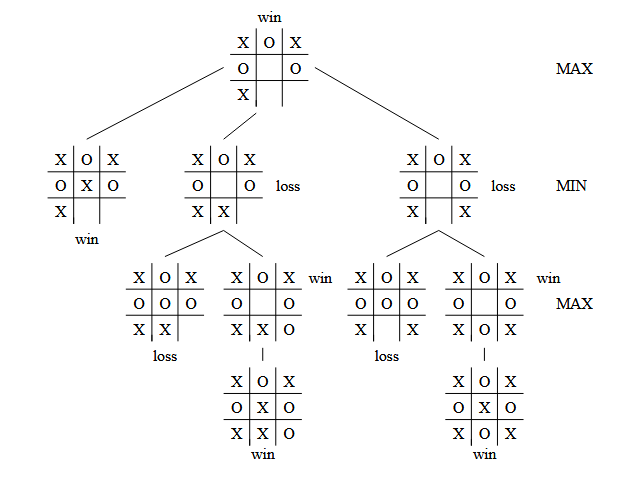
\includegraphics[width=0.7\textwidth]{images/ticTacToe.png}
    \caption{Possible plays for Tic Tac Toe}
    \label{fig:ticTacToe}
\end{figure}

\begin{figure}
    \centering
    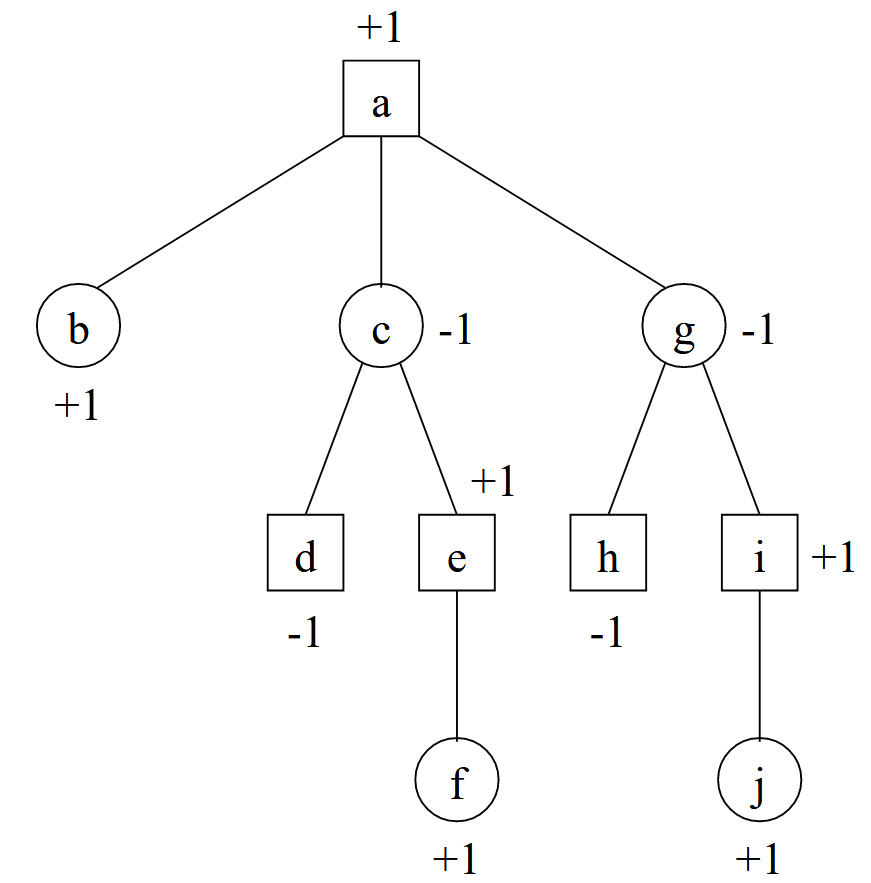
\includegraphics[width=0.7\textwidth]{images/minimax.png}
    \caption{Minimax Tree for Tic Tac Toe}
    \label{fig:minimax}
\end{figure}

\begin{algorithm}[h]
    \caption{Minimax Algorithm}
    \begin{algorithmic}
        \Function{Minimax}{Node, Depth, MaximizingPlayer}
        \If{Depth = 0 or Node = Leaf}
        \State \Return \Call{Eval}{Node}
        \EndIf
        \If{MaximizingPlayer}
        \State $Value \gets -\infty$
        \For{each  in Node}
        \State $Value \gets \max(value, \textsc{Minimax}(\textit{child}, \textit{depth} - 1, \textbf{false}))$
        \EndFor
        \State \Return $Value$
        \Else
        \State $Value \gets \infty$
        \For{each Child in Node}
        \State $Value \gets \min(value, \textsc{Minimax}(\textit{child}, \textit{depth} - 1, \textbf{false}))$
        \EndFor
        \State \Return $Value$
        \EndIf
        \EndFunction
    \end{algorithmic}
\end{algorithm}


Alpha-Beta pruning is a an approach used to decrease the number of nodes evaluated by the minimax algorithm.
It does this by not evaluating nodes that would not affect the final outcome of the minimax algorithm.
It introduces two new values $\alpha$ and $\beta$ where $\alpha$ represents the maximum value
that can be attained and $\beta$ represents the minimum value that can be attained. If the 
value of a node is less than $\alpha$ or greater than $\beta$, the tree does not need to be
traversed further.


\subsection{Naive Bayes}
\label{sec:naivebayes}
Many Machine Learning algorithms have been used in chess engines. The most popular being Neural Networks
like used in AlphaZero \cite{kleinNeuralNetworksChess2022}. Another popular technique is using reinforcement
learning where the engine plays against itself and learns from the results \cite{silverGeneralReinforcementLearning2018}.
Naive Bayes hasn't been as popular in chess engines. Naive Bayes, sometimes also known as Idiot Bayes or Simple Bayes,
is a simple classification algorithm that utilises Bayes' theorem (Equation~\ref{eq:bayestheorem}).\cite{lowdNaiveBayesModels2005}. 

\begin{equation}
    \label{eq:bayestheorem}
    P(A|B) = \frac{P(B|A) \cdot P(A)}{P(B)}
\end{equation}
It is referred to as naive as it assumes that each input variable $X_1, X_2,..., X_n $ is conditionally independent given the classDespite this assumption not being true in most cases, Naive Bayes has
still been shown to work well. This assumption allows probability distributions to be efficiently represented
as the product of the individual probabilities of the input variables (Equation~\ref{eq:naivebayes}) \cite{lowdNaiveBayesModels2005}.
\begin{equation}
\label{eq:naivebayes}
P(X_1, X_2, ..., X_n, C) ={P(C)}\cdot \prod_{i=1}^{n}{P(X_i | C)}
\end{equation}

Naive Bayes has been shown to be effective in many domains, for example in spam detection \cite{eberhardtBayesianSpamDetection2015}.
Some academics from Jaypee Institute of Information Technology compared between two different
techniques, Naive Bayes Classification and Multivariate Linear Regression. They found that Naive Bayes
was better suited for categorical predictions while Multivariate Linear Regression struggled with
predictions \cite{departmentofcomputerscienceandengineeringjaypeeinstituteofinformationtechnologynoida201304indiaStatisticalAnalysisResult2018}


\section{Requirements}

\subsection{Functional Requirements}
\label{sec:functional}
\begin{itemize}
    \item The system must evaluate chess positions using a Naive Bayes Classifier.
    \item The classifier should be able to output a classification for a position. (Winning, Losing, Drawing)
    \item The evaluation should be integrated with Minimax and Alpha-Beta pruning.
    \item The engine should be able to play a full game of chess.
    \item The engine should be able to evaluate the board position.
    \item The engine should be able to make a move based on the evaluation.
\end{itemize}

\subsection{Non-Functional Requirements}
\label{sec:nonfunctional}
\begin{itemize}
    \item The classifier should be computationally efficient for real time evaluation.
    \item The classifier should be scalable to handle large datasets.
    \item The system should be able to evaluate a position in less than 4 second.
    \item The system should be able to run on a standard laptop.
    \item The system should be testable against Stockfish.
\end{itemize}




\section{Methodology}
\label{sec:methodolgy}

\subsection{Problem Definition}
\label{sec:problem}
Naive Bayes has been proven to work in certain domains, this research aims to see if it can be 
effective in a chess engine. The system will be implemented in Python, utilising the python-chess package
for board representation and move generation. The Naive Bayes classifier will be trained to categorise
chess positions into 3 categories, Winning, Losing, and Drawing. The classifier will be used within the
minimax algorithm to then help decide which nodes to evaluate further and which to terminate at.

\subsection{Data Collection and Representation}
\label{sec:data}
The classifier will be trained on a dataset of chess positions. The dataset that will be used 
is from the lichess database. This database contains over six billion games of chess. Due to 
constraints on computational power as well as time, only a subset of this database will be used.
Due to the nature of Naive Bayes, the dataset will need to be preprocessed to include two main parts, 
the features and the labels/classes. The labels is what the classifier will predict. We will 
use three labels for the classifier:
\begin{itemize}
    \item Winning
    \item Losing
    \item Drawing
\end{itemize}

The features are the input variables that will be used 
for the classifier since Naive Bayes is a supervised learning algorithm which require numerical 
or categorical features to calculate the conditional probabilities of the labels. These features
are the "evidence". For the purpose of this research, the following features will be used:

\subsubsection{Material Balance}
\label{sec:material}
The material balance is arguably the most important feature in chess. Material balance is the
difference between the number of white pieces and the number of black pieces refer to Equation~\ref{eq:material}.
This feature is a good indicator of the current standing of the game. The material balance is 
positive if White has more pieces than Black and negative if Black has more pieces than White,
and 0 otherwise.
\begin{equation}
    \label{eq:material}
    \text{Material Balance} = \text{Number of White Pieces} - \text{Number of Black Pieces} 
\end{equation}


However, considering each piece of equal value is not representative of the true value of pieces
during the game, for example arguably 1 queen is worth more than 2 pawns. Keeping this in mind,
this research will use the values in Table \ref{tab:values} to calculate the material balance,
which are the commonly accepted values of pieces in chess\cite{guptaDeterminingChessPiece2023}.
Many other values have been proposed, however, this research will use these values as they are
the most commonly accepted. 

\begin{table}[h]
    \centering
    \begin{tabular}{|c|c|}
        \hline
        \textbf{Piece} & \textbf{Value} \\
        \hline
        Pawn & 1 \\
        Knight & 3 \\
        Bishop & 3 \\
        Rook & 5 \\
        Queen & 9 \\
        King & 0 \\
        \hline
    \end{tabular}
    \caption{Values of Chess Pieces}
    \label{tab:values}
\end{table}





\subsubsection{King Safety}
\label{sec:kingsafety}
Material Balance is a very good indicator of the current standing of the game, however, it does not
consider anything related to the king, which could single handedly change the outcome of the game. King
Safety is a feature that will be used to evaluate the safety of the king. Again, there are many proposed
methods to evaluate the safety of the king \cite{KingSafetyChessprogramming}, however, this research will 
calculate King Safety solely based on the number of pieces attacking the king.


\subsubsection{Piece mobility}
\label{sec:mobility}
Another drawback of relying solely on material balance, is that it doesn't consider the state of the game, if you have the 
same pieces in two games, the material balance would be the same, however, the state of the game could be very different.
One way of tackling this issue is introducing the idea of piece mobility. Piece mobility is the number of legal moves a piece
can make. The more mobility one side has, generally indicates they have more control over the board. This feature will be the 
difference of the number of legal moves White has and the number of legal moves Black has as shown in Equation~\ref{eq:mobility}.

\begin{equation}
    \label{eq:mobility}
    \text{Mobility} = \sum_{i=1}^{n} \text{LegalMoves}_i^{\text{White}} - \sum_{j=1}^{m} \text{LegalMoves}_j^{\text{Black}}
\end{equation}


\subsubsection{Pawn Structure}
\label{sec:pawnstructure}
Despite being the weakest piece in chess, pawns can be instrumental in the progression of the game
due to their ability to control the centre of the board and being able to promote to another piece. 
There are 3 main pawn structures that we will consider. Doubled pawns, isolated pawns, and passed pawns
\cite{PawnStructureChessprogramming}.

\begin{itemize}
    \item \textbf{Doubled Pawns}: Doubled pawns are two pawns of the same colour that are on the same file.
    They are usually seen as weak since they can't defend each other and can be easily attacked.
    \item \textbf{Isolated Pawns}: Isolated pawns, also known as isoloni pawns, are pawns that do not have
    any friendly pawns on adjacent files. They are also considered weak as they can't be protected by other pawns
    \item \textbf{Passed Pawns}: Passed pawns are pawns that have advanced past all opposing pawns \cite{PassedPawnChesscom}.
    In other words they have no enemy pawns in front of them or on adjacent files that can stop them from 
    being promoted \cite{PassedPawnChesscom}. Unlike doubled and isolated pawns, passed pawns are considered
    strong as they can be easily promoted to a queen, forcing the opponent to use their pieces to stop that pawn.
\end{itemize}



\subsubsection{Control of the Centre}
Another important feature is to consider the control of the centre. Having control of the centre 
is a strong advantage as it allows for more mobility and more options for the player \cite{mikhalchishinCentreModernStrategy}. This will be evaluated
by calculating the number of pieces in the centre of the board and taking the difference between the
number of white pieces and the number of black pieces. The centre of the board is defined by the 16 squares
in the middle of the board (Figure~\ref{fig:bigcentre}), giving more weight to the 4 squares in the centre (Figure~\ref{fig:smallcentre}).


\begin{figure}[h]
    \centering
    \begin{subfigure}[b]{0.4\textwidth}
        \centering
        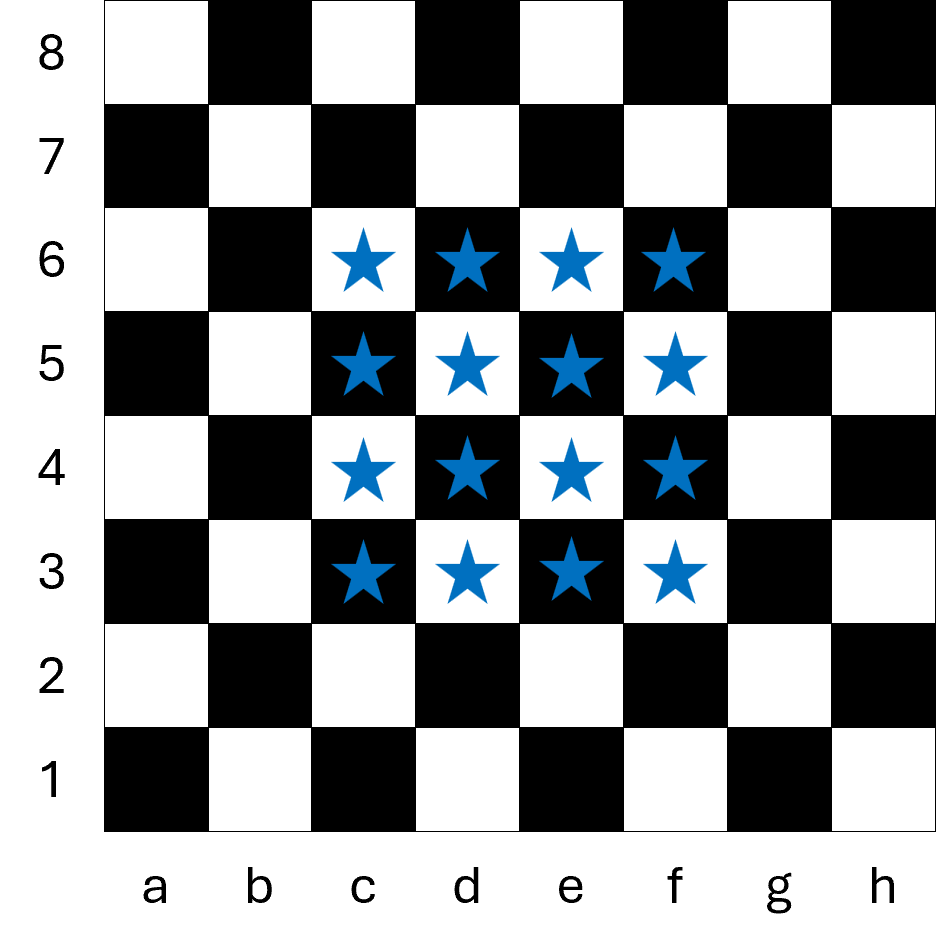
\includegraphics[width=\textwidth]{images/bigCentre.png}
        \caption{Big centre of the Board}
        \label{fig:bigcentre}
    \end{subfigure}
    \hfill
    \begin{subfigure}[b]{0.4\textwidth}
        \centering
        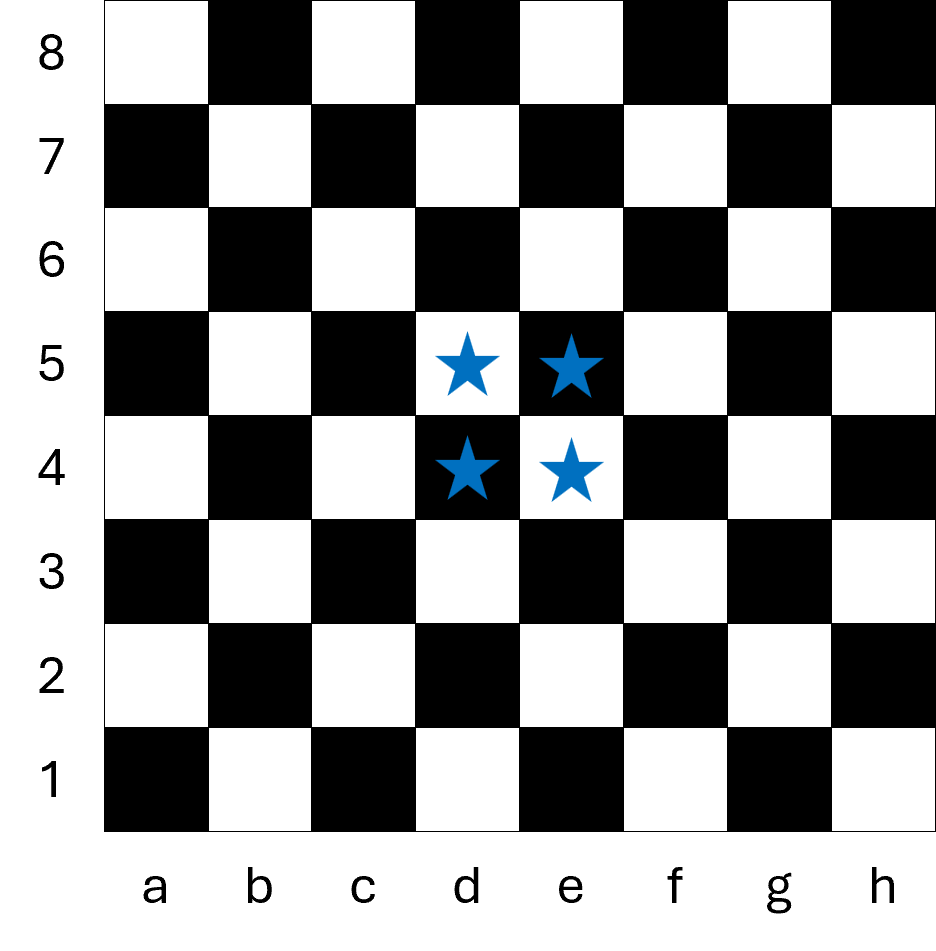
\includegraphics[width=\textwidth]{images/smallCentre.png}
        \caption{Small centre of the Board}
        \label{fig:smallcentre}
    \end{subfigure}
    \caption{Comparison of the small and big centres of the board.}
    \label{fig:centres}
\end{figure}




\subsection{Training the Classifier}
\label{sec:training}
Once the data has been collected and preprocessed, the classifier can be trained. There is the input data
and the labels/classes that the input data will be classified into.
The data will be split into training data and testing data, with a 80\%/20\% split respectively. 

\subsubsection{Prior Probabilities}
\label{sec:prior}
The first step 
is to calculate the prior probabilities of the classes, which is based on the training data. Equation~\ref{eq:prior}
shows how it is calculated, where $C$ is the class, $N_c$ is the number of instances of the class and $N$ is the 
total number of instances in the training data.

\begin{equation}
    \label{eq:prior}
    P(C) = \frac{N_c}{N}
\end{equation}


\subsubsection{Likelihood Probabilities}
\label{sec:likelihood}
The likelihood probability, $P(X | C)$, involves calculating the probability distribution of each feature given a class.
There are 2 main types of Naive Bayes classifiers, Gaussian Naive Bayes and Multinomial Naive Bayes. Gaussian Naive Bayes
is used for continuous features so calculates the likelihood probability using a Gaussian Normal Distribution (Equation
\ref{eq:gaussian}).
\begin{equation}
    \label{eq:gaussian}
    P(X | C) = \frac{1}{\sqrt{2\pi\sigma^2}}e^{-\frac{(X-\mu)^2}{2\sigma^2}}
\end{equation}

\begin{itemize}
    \item $X$: Feature
    \item $\mu$: Mean of the feature
    \item $\sigma$: Standard Deviation of the feature
\end{itemize}

Multinomial Naive Bayes is used for discrete features so calculates the likelihood based on 
the count of feature in the class (Equation~\ref{eq:multinomial}). 

\begin{equation}
    \label{eq:multinomial}
    P(X | C) = \frac{N_{X,C} + 1}{N_C + V}
\end{equation}

\begin{itemize}
    \item $N_{X,C}$: Number of instances of the feature $X$ in class $C$
    \item $1$: Laplace smoothing constant
    \item $N_C$: Number of instances in class $C$
    \item $V$: Number of possible values for $X$
\end{itemize}

For this research we use features that are continuous and discrete, so we will use both Gaussian and Multinomial Naive Bayes
and then evaluate which one fits better for the data.

\subsubsection{Posterior Probabilities}
\label{sec:posterior}
Now that we have the prior and likelihood probabilities we can use Bayes' Theorem to calculate the posterior probabilities.

\begin{equation}
    \label{eq:posterior}
    P(C | X) = \frac{P(X | C) \cdot P(C)}{P(X)}
\end{equation}

P(X) is considered the ``evidence'' and is the same for all the classes so can be ignored when
comparing the posterior probabilities.
To calculate the predicted class for a given instance, we choose the class with the highest posterior probability
as shown in Equation~\ref{eq:predict}.

\begin{equation}
    \label{eq:predict}
    Predicted Class = \arg\max_{C} P(C | X)
\end{equation}

\subsubsection{Evaluation}
\label{sec:evaluation}
The classifier will be then evaluated using the testing data. We will use accuracy and $f_1$ score as 
the evaluation metrics The accuracy is the ratio of correct predictions to total predictions and the $f_1$ score
is the harmonic mean of precision and recall. 

\begin{equation}
    \label{eq:accuracy}
    \text{Accuracy} = \frac{\text{Number of Correct Predictions}}{\text{Total Number of Predictions}}
\end{equation}

\begin{equation}
    \label{eq:precision}
    \text{Precision} = \frac{\text{TP}}{\text{TP} + \text{FP}}
\end{equation}

\begin{equation}
    \label{eq:recall}
    \text{Recall} = \frac{\text{TP}}{\text{TP} + \text{FN}}
\end{equation}

\begin{equation}
    \label{eq:f1}
    f_1 =  \frac{1}{\text{Precision}^{-1} + \text{Recall}^{-1}}
\end{equation}


\subsection{Integration with Minimax}
\label{sec:integration}
We now want to integrate the classifier into the minimax algorithm. The classifier's output will be used 
during the evaluation phase of each node. The classifier will output the probability of winning, losing, or Drawing
for a given game state. Using this a single score will be calculated.

\begin{equation}
    \label{eq:score}
    \text{ClassifierScore(X)} = P(\text{Winning}|X) - P(\text{Losing}|X)
\end{equation}

Then this score will be used in conjunction with a traditional evaluation function to evaluate 
a overall score, which will inform which nodes to evaluate further and which to terminate at.



\bibliographystyle{ieeetr}
\bibliography{references}
\end{document}
